\documentclass{article}
\usepackage[a4paper, margin=1in]{geometry}
\usepackage{graphicx}
\usepackage{hyperref}
\usepackage{polski}
\usepackage{float}

\title{Sztuczna inteligencja i inżyniera wiedzy\\
        Sprawozdanie z laboratorium 1}
\author{Patryk Łuszczek \\
        Numer indeksu: 272707
        \\ Grupa 1}
\date{\today}

\begin{document}

\maketitle

\section{Zadanie 1}
\subsection*{Graf i wprowadzenie danych}
W celu zrealizowania zadania, został stworzony graf na podstawie danych dostarczonych w ramach zadania.
Grał bazuje na implementacji grafu wielokrotnie skierowanego z biblioteki NetworkX i rozszerza go o dodatkowe funkcjonalności takie jak np. znajdowanie najlepszego połączenia z uwzględnieniem zmiennych kryteriów, oraz normalizacją
danych przy ich ładowaniu. Wierzchołek reprezentuje pojedynczy przystanek wraz z jego danymi geolokacyjnymi. W celu uproszczenia, przystanki o tej samej nazwie są traktowane jako jeden wierzchołek, czas podróży oraz odległości między takimi przystankammi były na tyle niewielkie,
że nie wpłwa to na jakość działania algorytmów.

\begin{figure}[H]
    \centering
    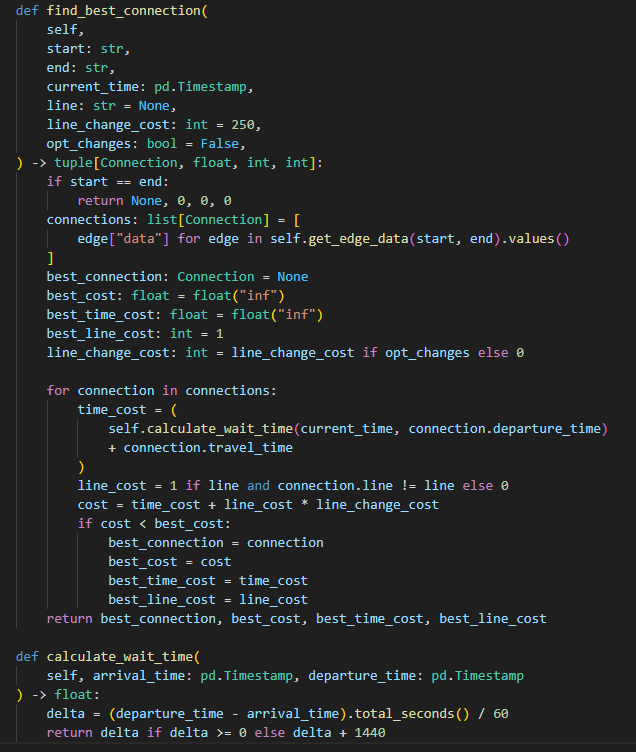
\includegraphics[width=0.7\textwidth]{sc1.png}
\end{figure}

Została utworzona dataklasa \texttt{Connection} reprezentująca połączenia w grafie, która zawiera niezbędne informacje tj. linia oraz czas podróży.

\begin{figure}[H]
    \centering
    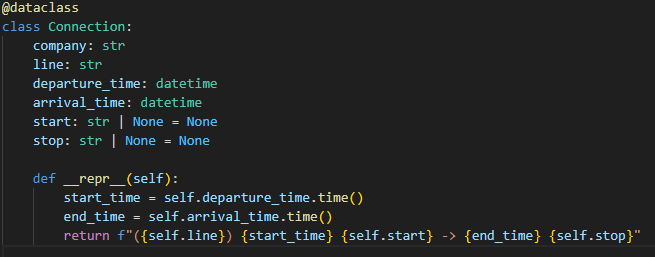
\includegraphics[width=0.7\textwidth]{sc2.png}
\end{figure}



\subsection*{Algortytm Dijkstry}
Algorytm Dijkstry służy do znajdowania najkrótszej ścieżki. Opiera się na kolejce priorytetowej, w której znajdują się następne wierzchołki do odwiedzenia, a ułożone są według wyliczonych wcześniej wag. Początkowo
znajduje się w niej wyłącznie wierzchołek początkowy o wadze równej zero, następnie odwiedzane są sąsiednie wierzchołki, a ich wagi są ustalane jako waga wierzchołka, z którego zostały odwiedzone oraz waga krawędzi, tj. połączenia. Z racji, że
między dwoma wierzchołkami może występować wiele krawędzi, wybierana jest ta najlepsza, zgodnie z kryterium optymalizacji, tutaj czasem podróży. Następnie wierzchołek jest dodawany do kolejki, a algorytm działa dopóki
nie dotrze do wierzchołka docelowego lub kolejka nie będzie pusta. W momencie dotarcia do wierzchołka docelowego, algorytm kończy działanie i zwraca najkrótszą ścieżkę oraz czas podróży.


\subsection*{Algorytm A*}
Algorytm A* jest również algorytmem służącym do znajdowania najkrótszej ścieżki, jednak w odróżnieniu od Dijkstry wykorzystuje dodatkowo heurystykę,
która umożliwia szacowanie pozostałego kosztu dla danego węzła. Dzięki temu, algorytm może działać szybciej, jednak rozwiązanie może nie zawsze być optymalne.
Jako heurystykę wykorzystałem obliczenie pozostałego czasu podróży na podstawie danych lokalizacyjnych przystanków. Jeśli optymalizowana jest liczba przesiadek, to jest sprawdzane czy
obecnie rozpatrzane połączenie może zawierać się w połączeniach przychodzących do celu na podstawie linii. W przypadku moich algorytmów, implementacyjnie A* niewiele różni się od Dijkstry, z wyjątkiem wykorzystania właśnie dodatkowego kroku
obliczenia heurystyki.

\begin{figure}[H]
    \centering
    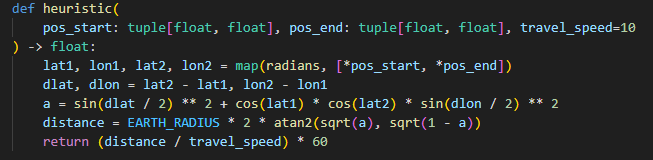
\includegraphics[width=0.7\textwidth]{sc3.png}
\end{figure}

Oba algorytmy wykorzystują funkcję kosztu polegającą na obliczeniu czasu oczekwiania na dotarcie do przystanku, uwzględniając czas podróży oraz czas oczekiwania na polączenie. Dodatkowo, jeśli
optymalizowana jest liczba przesiadek, to kara za przesiadkę jest dodawana do całkowitego kosztu.

\subsection*{Wnioski}
Dla przykładowych danych testowych tj:
\begin{verbatim}
    start = 'Tarnogaj'
    end = 'Pl. Wróblewskiego'
    time = '12:00:00'
\end{verbatim}
Zbadano wyniki działania obu algorytmów:
\begin{figure}[H]
    \centering
    \includegraphics[width=0.7\textwidth]{sc4.png}
    \caption{Wyniki działania algorytmu Dijkstry}
\end{figure}

\begin{figure}[H]
    \centering
    \includegraphics[width=0.7\textwidth]{sc5.png}
    \caption{Wyniki działania algorytmu A*}
\end{figure}





Dodatkowo, na tej samej trasie została wykorzystana opcja optymalizacji liczby przesiadek dla algorytmu A*.
\begin{figure}[H]
    \centering
    \includegraphics[width=0.7\textwidth]{sc6.png}
    \caption{Wyniki działania algorytmu A* z optymalizacją liczby przesiadek}
\end{figure}
Jak można zauważyć, dla optymalizacji czasu podróży oba algorytmy znalazły te same połączenia. Algorytm A* znalazł je nieznacznie szybciej.
W przypadku optymalizacji przesiadek można zauważyć różnicę w trasie oraz kosztach tej trasy.

\section{Zadanie 2}
Do implementacji tabu search, wykorzsystałem działanie algorytmu A*, który porównuje koszt dla różnych kombinacji przystanków do odwiedzenia.
Tablica tabu jest dobierana na podstawie liczby przystanków do odwiedzenia, a sąsiedztwo oraz jego rozmiar jest obliczany na podstawie zmian kolejności w odniesieniu do obcnego rozwiązania.
Dodatkowo, jeśli od kilku iteracji nie znaleziono lepszego rozwiązania, to przeszukiwane jest większe sąsiedztwo. Wykorzystana została również aspiracja, która pozwala na
zignorowanie tabu. Wartość aspiracji jest ustalana na podstawie obecnie najlepszego kosztu, oraz wartości zmian jakie zachodziły w poprzednich iteracjach.
\begin{figure}[H]

    \centering
    \includegraphics[width=0.7\textwidth]{tabu.png}
    \caption{Fragment kodu tabu search}
\end{figure}


Dla przykłądowych danych testowych tj:
\begin{verbatim}[H]
    start = 'Gaj'
    time = '12:00:00'
    stops = ['Dworzec Autobusowy','Galeria Dominikańska,'Rynek,'Dworzec Główny']
\end{verbatim}
Zoptymalizowano czas podróży oraz liczbę przesiadek. Co ciekawe oba tryby optymalizacji znalazły połączenia, które
skutykowały tym samym czasem podróży, jednakże optymalizacja przesiadek zmniejszyła łączną liczbę przesiadek o 4.

\begin{figure}[H]

    \centering
    \includegraphics[width=0.7\textwidth]{sc7.png}
    \caption{Wyniki działania algorytmu Tabu Search z optymalizacją czasu podróży}
\end{figure}

\begin{figure}[H]
    \centering
    \includegraphics[width=0.7\textwidth]{sc8.png}
    \caption{Wyniki działania algorytmu Tabu Search z optymalizacją liczby przesiadek}
\end{figure}

Jak można zauważyć, optymalizacja przesiadek znalazła rozwiązanie z mniejszą liczbą przesiadek. Jest to rozwiązanie dostatecznie dobre, ponieważ zapewne całość trasy mogła być zrealizowana
za wykorzystaniem jednej linii autobusowej. Wyniki kosztu zmian linii, przez moje niedopatrzenie, zostało policzone jako łączenie indywidualnych kosztów między przystankami w trasie (wartość zwracana przez stosowanie
algoroytmu A*).

\section*{Wnioski}
W wyniku rozwiązywania zadania, udało mi się zaimplementować algorytmy znajdujące najlepsze trasy w oparcu o kryterium przesiadek lub czasu podróży.
Takie rozwiązanie bardzo przypomina działanie aplikacji jak Google Maps czy Jakdojadę, które prawdopodobnie wykorzystują podobne algorytmy.
Największym wyzwaniem było zaimplementowanie efektywnego algorytmu Tabu Search, który po wielu próbach optymalizacji wciąż zajmuje trochę czasu na obliczenie.
Wiąże się to oczywiście z wieloma przypadkami i kombinacjami do rozpatrzenia. Algorytmy A* oraz Dijkstry działają bardzo szybko, a ich czas działania rośnie proporcjonalnie do
odległości między przystankiem końcowym a początkowym.




\end{document}
